\documentclass[12pt, a4paper]{scrreprt}

% Pacotes básicos
\usepackage[utf8]{inputenc}
\usepackage[portuguese]{babel}
\usepackage{geometry}
\usepackage{hyperref}
\usepackage{graphicx}
\usepackage{svg}
\usepackage{amsmath}

% Pacotes para citações
\usepackage{csquotes}
\usepackage[backend=biber,style=numeric]{biblatex} 
\addbibresource{referencias.bib} % Nome do arquivo .bib

\usepackage{helvet} % Similar à Arial
\renewcommand{\familydefault}{\sfdefault} % Sans-serif

% Define o espaço entre parágrafos
\setlength{\parskip}{1em} % Ajuste o valor conforme necessário
\setlength{\parindent}{0pt} % Sem recuo

% Configurações de margens
\geometry{left=2cm, right=2cm, top=2cm, bottom=2cm}

% Configurações de cabeçalhos e rodapés
\usepackage{scrlayer-scrpage}
\pagestyle{scrheadings}

% Definições de cabeçalhos e rodapés
\ihead{Árvores}
\chead{\leftmark}
\ohead{\pagemark}

% Início do documento
\begin{document}
\begin{titlepage}
    \centering
    \begin{figure}[h]
        \centering
        
\includegraphics[width=.75\textwidth]{src/logo_unesp.jpg}
        \label{fig:logo_unesp}
    \end{figure}
    \vfill
    \Huge\textbf{Relatório de estudo sobre grafos do \\ tipo árvore}\\[1.5cm]
    \Large\textbf{Grafos e Aplicações}\\[1.5cm]
    \vfill
    \begin{flushleft}
        \textbf{Equipe:}\\
        \hspace{1.5cm}André Luis Dias Nogueira \\ 
        \hspace{1.5cm}Felipe Melchior de Britto \\
        \hspace{1.5cm}Rafael Daiki Kaneko \\
        \hspace{1.5cm}Ryan Hideki Tadeo Guimarães \\
        \hspace{1.5cm}Vitor Marchini Rolisola \\
    \end{flushleft}
    \vfill
    01/08/2024\\
\end{titlepage}

% Sumário
\tableofcontents
\newpage

% Resumo
\chapter{Resumo}

Este trabalho tem como objetivo aplicar o algoritmo de Busca em Largura (BFS) em árvores binomiais geradas aleatoriamente, calculando a média das profundidades das ordenações geradas para todos os nós. O número de filhos por nó segue uma distribuição binomial com parâmetros \( n_{\text{max}} \) (número máximo de filhos) e \( p\) (probabilidade de ter filhos), sendo a geração de descendentes limitada pela profundidade \( d_{\text{max}} \).

Realizamos experimentos variando os parâmetros \( n_{\text{max}} \), \( p \), e \( d_{\text{max}} \), gerando ao menos 10 árvores aleatórias para cada combinação de valores. Os resultados obtidos foram apresentados em tabelas e gráficos, permitindo a análise das profundidades médias.

Um dos interesses do estudo era almejar a transição de fase esperada no modelo: para \( n_{\text{max}} \cdot p < 1 \), as árvores atingem no geral níveis sem descendentes enquanto para \( n_{\text{max}} \cdot p > 1 \), as árvores se expandem até o limite de profundidade \( d_{\text{max}} \). Esse comportamente fornece uma visão mais detalhada sobre a estrutura de crescimento das árvores binomias conforme variamos seus parâmetros.

% Introdução
\chapter{Introdução}

Grafos são estruturas fundamentais em teoria dos grafos, utilizadas para modelar uma variedade de problemas em diferentes áreas, desde redes de computadores até genética.

Um grafo é uma estrutura matemática usada para modelar relações entre objetos de um conjunto. Ele é composto por dois conjuntos: um conjunto de vértices (ou nós) e um conjunto de arestas (ou arcos) que conectam esses vértices. Os vértices representam os objetos e as arestas representam as relações entre esses objetos. \textsuperscript{\cite{emilio2024grafos}}

\begin{figure}[h]
    \centering
    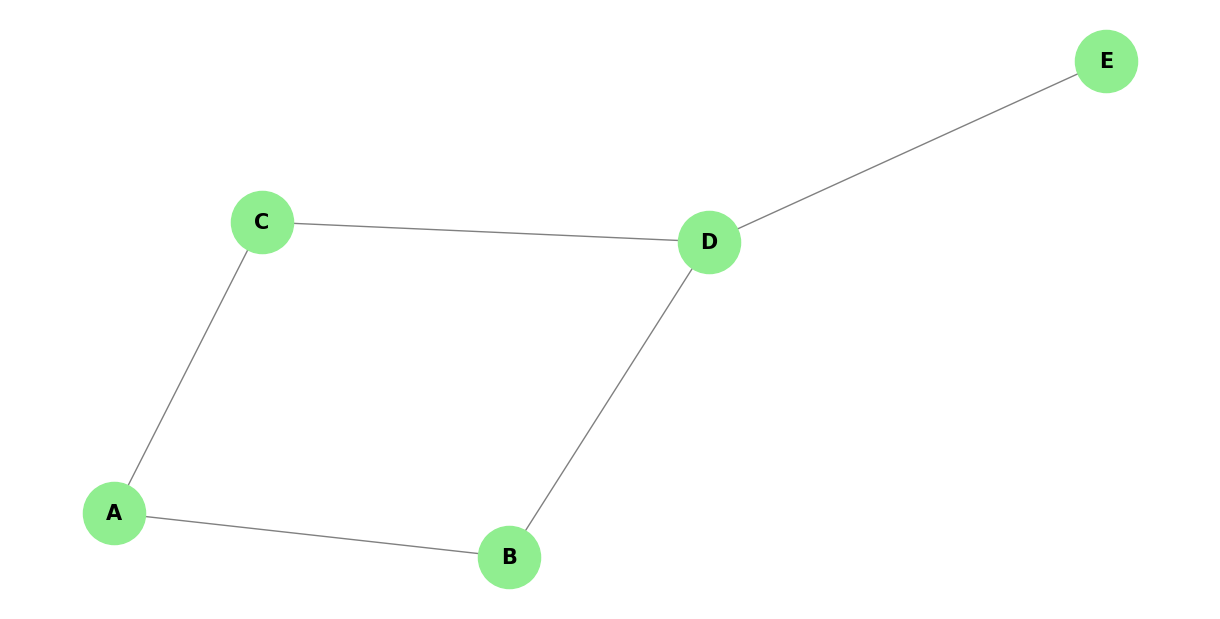
\includegraphics[width=.75\textwidth]{src/exemplo_simples_grafo.png}
    \label{fig:exemplo de grafo simples}
\end{figure}

Por exemplo, na representação de uma rede social, os vértices podem representar pessoas e as arestas representam as conexões de amizade entre elas.

Um tipo especial de grafo, conhecido como árvore, apresenta propriedades únicas que tornam essa classe particularmente interessante para estudo.

Uma árvore é definida como um grafo não-orientado, conexo e acíclico, o que significa que não possui ciclos e, além disso, qualquer remoção de uma de suas arestas resulta em um grafo desconexo.\textsuperscript{\cite{definicaoarvore}} Então suas características são:

\begin{itemize}
        \item \textbf{Conectividade}: Para qualquer par de vértices \( u \) e \( v \), existe exatamente um caminho que conecta \( u \) e \( v \).
        \item \textbf{Aciclicidade}: O grafo não contém ciclos; ou seja; não é possivel iniciar em im vértice, seguir arestas e retornar ao mesmo vértice sem atravessar arestas repetidamente.
        \item \textbf{Número de arestas}: Se uma árvore possui \( n \) vértices, então ela possui exatamente \( n - 1 \) arestas.
\end{itemize}

\begin{figure}[h]
    \centering
    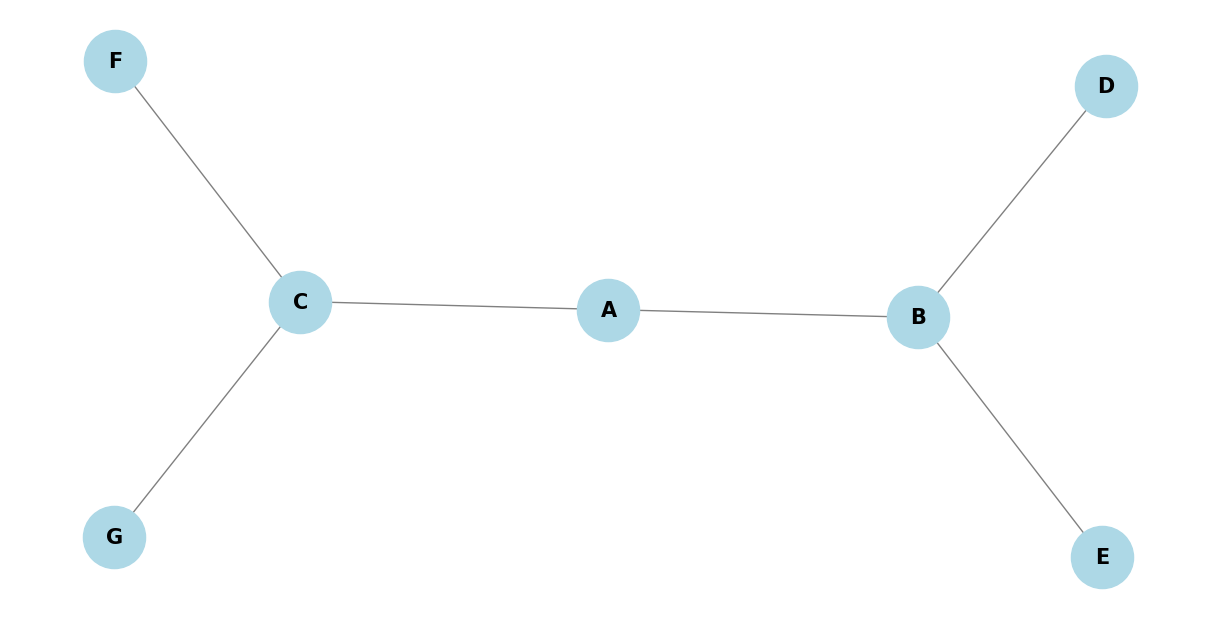
\includegraphics[width=.65\textwidth]{src/arvore_exemplo.png}
    \label{fig:exemplo de árvore}
\end{figure}

Essas características permitem que árvores sejam a estrutura mínima necessária para garantir a conectividade entre os vértices de um grafo com o menor número de arestas possíveis, um aspecto crucial para a otimização de recursos em diversos cenários práticos.

A análise de árvores em grafos tem implicações diretas em problemas de interligação, como o fornecimento de redes elétricas, onde o objetivo é minimizar o custo de conexão ao garantir que todas as unidades estejam conectadas. Além disso, árvores desempenham um papel importante na computação, particularmente em algoritmos de ordenação, como o Heapsort, e na modelagem de genealogias e redes hierárquicas.

Uma \textbf{árvore binomial} é uma estrutura de dados que representa uma coleção de árvores binomiais. A definição formal de uma árvore binomial é a seguinte\textsuperscript{\cite{definicaoarvorebinomialEllis} \cite{definicaoarvorebinomialTarjan}}:

Uma \textbf{árvore binomial} \( B_k \) é uma árvore que possui as seguintes propriedades:

\begin{itemize}
    \item \textbf{Estrutura Recursiva}: Uma árvore binomial \( B_k \) é composta por \( 2^k \) nós e tem exatamente \( k \) árvores binomiais \( B_{k-1}, B_{k-2}, \ldots, B_0 \) como subárvores. A árvore \( B_k \) é obtida ao unir duas árvores \( B_{k-1} \).
    
    \item \textbf{Propriedades dos Nós}: 
    \begin{itemize}
        \item O nó na raiz de \( B_k \) tem um grau de \( k \) (ou seja, ele possui \( k \) filhos).
        \item A altura de \( B_k \) é \( k \).
        \item A árvore \( B_k \) possui \( 2^k \) folhas.
    \end{itemize}
    
    \item \textbf{Organização dos Nós}: Os nós são organizados de tal forma que os valores dos nós na subárvore esquerda são menores ou iguais ao valor do nó pai, e os valores dos nós na subárvore direita são maiores.
\end{itemize}

\begin{figure}[h]
    \centering
    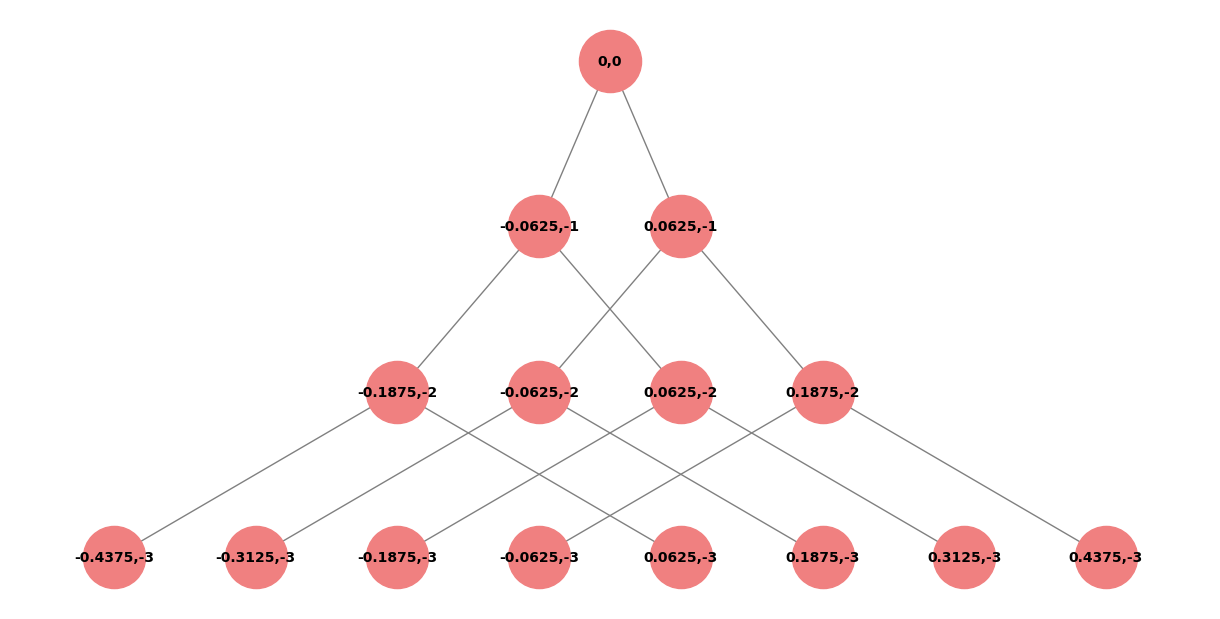
\includegraphics[width=.72\textwidth]{src/arvore_binomial_ordem_3.png}
    \label{fig:exemplo de árvore binomial}
\end{figure}

As árvores binomiais são particularmente úteis em algoritmos de estrutura de dados, como em filas de prioridade.

O presente relatório tem o objetivo de explorar as propriedades matemáticas e aplicativas das árvores binomiais, abordando tanto sua definição formal quanto suas extensões, como arborescências e a aplicação em algoritmos de busca.

A introdução a essas ideias será contextualizada com base nas propriedades da conectividade e da aciclicidade, discutindo ainda como árvores binomiais podem ser vistas como estruturas mínimas e otimizadas para representação de relações complexas, ao mesmo tempo que mantêm a simplicidade computacional.

% Implementação
\chapter{Implementação}
A implementação do trabalho envolve a criação de um algoritmo que gera árvores binomiais com base nos parâmetros fornecidos: \( n_{\text{max}} \) (número máximo de filhos por nó), \( p \) (probabilidade de um nó gerar filhos) e \( d_{\text{max}} \) (profundidade máxima da árvore). Cada nó é representado por um conjunto de quatro posições em um vetor. A primeira posição do vetor, exclusivamente, armazena o número máximo de filhos do nó, enquanto as outras três posições armazenam o índice do pai e dos filhos, respectivamente, conforme o modelo que você está utilizando.

Para cada tripla de parâmetros, são geradas pelo menos 10 árvores aleatórias, utilizando a distribuição binomial para decidir quantos filhos cada nó terá. O algoritmo segue uma abordagem de Busca em Largura (BFS) para explorar os nós da árvore. A BFS percorre a árvore começando da raiz, explorando todos os nós em cada nível antes de passar para o próximo. Essa busca é gerenciada por uma fila que armazena os nós a serem explorados, garantindo que os nós sejam processados em ordem de nível.

Durante a execução do BFS, são registrados a profundidade de cada nó e a profundidade total das árvores. Ao final de cada execução, é calculada a profundidade média da árvore, que será utilizada para gerar tabelas ou gráficos que mostram como essa profundidade varia de acordo com as diferentes combinações de \( n_{\text{max}} \), \( p \), e \( d_{\text{max}} \).

Além disso, o código precisa lidar com a transição de fase do modelo, que ocorre quando nmax multiplicado por p é menor que 1, indicando que, em algum ponto, a geração de novos filhos para a árvore vai parar, resultando em níveis sem descendentes. Caso \( n_{\text{max}} \cdot p \) seja maior que 1, a geração de nós continuará até atingir o limite imposto por \( d_{\text{max}} \).

Portanto, a implementação é construída de maneira a não apenas gerar as árvores e calcular as profundidades, mas também simular a dinâmica de crescimento dessas árvores binomiais sob diferentes condições, explorando a variação desses parâmetros.

% Resultados e discussão
\chapter{Resultados e discussão}

% Conclusão
\chapter{Conclusão}

% Referências bibliográficas
\printbibliography % Para imprimir a bibliografia


%Imagens da Introdução: Geradas com código no repositório: \href{https://github.com/FelipeMDB-UNESP/Grafos.git}{\cite{felipemdb2024}}.

\end{document}